\chapter{Elektrisk Felt}
  \section*{Coulombs lov}
    Coulombs lov sier at hvis en har to ladde partikkler vil det utøves en kraft som kan skrives slik:
    \[
    \frac{1}{4 π \epsilon_{0}} q ⋅ Q \frac{\hat{R}}{R^{2}}
    \]

    \begin{figure}[h!]
      \centering
      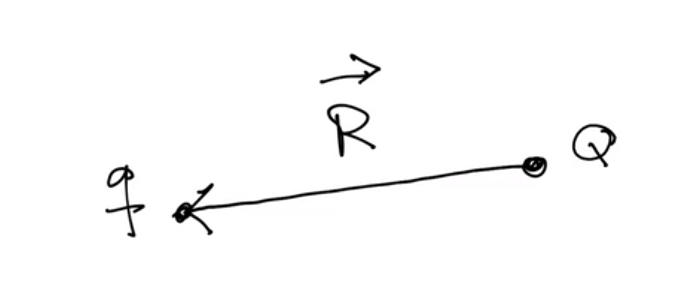
\includegraphics[scale = .7]{Bilder/Coulombs_lov.png}
      \caption{To ladde partikkler}
      \label{fig: Ladde partikkler}
    \end{figure}
  Ladning er en bevart størrelse og vil være konstant i et lukket system. \newline 

  \bf  Questions: The net force on a system due to all the electrostatic forces between charges in the system is zero. Is this statement true or false? Explain your answer. \newline \newline  
  
  \bf{True}: Kreftene vil kansellere hverandre i et større system selvom vi kan oppleve krefter lokalt. 

  